\documentclass[12pt]{report}  % if you want to use two side the code is following [12pt,twoside]
\usepackage[utf8]{inputenc}
\usepackage{graphicx}
\graphicspath{{images/}}
\usepackage{amsmath}
\usepackage{amssymb}
\usepackage{amsfonts}
\usepackage{subfig}
\usepackage{float}
\usepackage{nomencl}
\makenomenclature
\usepackage{multicol}
\usepackage[hidelinks]{hyperref}
\usepackage[a4paper,margin=1in,left=1.5in]{geometry}
\usepackage{setspace} % this packgae is for double spacing.
% to get the double spacing use \begin{doublespacing} and \end{doublespacing} in the section
\usepackage{fancyhdr}
%\usepackage[latin1]{inputenc}
\pagestyle{fancy}
\fancyhf{}
\fancyhead{} % to clear the header
\fancyfoot{} % to clear the footer
\fancyfoot[C]{\thepage}
%\fancyfoot[LE,RO]{\thepage}
%\fancyfoot[R]{\thepage\}, use this cmd instead
%\fancyfoot[LO,CE]{Chapter \thechapter}
% \fancyfoot[CO,RE]{Author Name}, this line will create another footer on bottom right
%to change the font size of header and footer the following command is useful
\renewcommand{\headrulewidth}{0pt} % if you want a line before the header put 1pt 
\renewcommand{\footrulewidth}{0pt} % if you want a line before the footer put 1pt 

\usepackage[backend=bibtex]{biblatex}
\addbibresource{reference.bib}
%\bibliography{reference.bib}
%\bibliographystyle{plain}
% this package is for appendix

%--------------------this package is for posting code in the latex
\usepackage{listings}

%---- these are for making the table of content


\begin{document}






\chapter*{Abstract}
\addcontentsline{toc}{chapter}{\numberline{}Abstract}
\begin{doublespacing}



\end{doublespacing}

\cleardoublepage
%----------------------------this is main matter
\pagenumbering{arabic}
\setcounter{page}{1}
\chapter{Introduction}
\section{Introduction}
\begin{doublespacing}
Thermal conductivity is one of the important properties in designing a nuclear fuel, since most of the physical phenomenon are thermally governed. In case of high-performance reactors, fuel goes through high fission density at relatively low temperatures. For this reason research reactor fuels are designed for efficient heat rejection. Usually it is composed of assemblies of thin-plates that uses aluminum alloy cladding. The Reduced Enrichment for Research and Test Reactors (RERR) program was initiated in the US in the late 1970s, to develop new fuels. This development of Low-Enriched Uranium (LEU) fuels for high-performence reactors is an important nonproliferatio initiatives~\cite{snelgrove1997development}. One of the major requirements is having higher Uranium density to offset the decrease in enrichment. Different alloys have been selected and tested. The U-Mo alloy has been identified as a high performence fuel due to its hgih Uranium density and low neutron capture cross-section~\cite{ewh2010microstructural,smirnova2013ternary,rest2009analysis,landa2013density}. During test operations, it was observed that thermal conductivity decreases with increased burnup. For a fission density of $3.30\times10^{21}$ fissions $cm^{-3}$, at $200^0C$ thermal conductivity decreases about $30\%$, for $4.53\times10^{21}$ fissions $cm^{-3}$ it becomes $45\%$~\cite{burkes2015thermal}. Fission also creates a variety of fission products. These fission products consists of gas bubbles, oxide precipitates, metallic precipitates and solid solution in the fuel matrix~\cite{rondinella2010high}. Radiation damage and fission products in reactor environment results in complex microstructure evolution which restructures the nuclear fuel over the period of time. Microsturctural evolution depends on the radial direction of the fuel~\cite{stehle1988performance,noirot2008detailed, meyer2014irradiation}. For every four fission events one inert gas atom (Xe or Kr) is produced. Xe atoms in U-Mo alloy fuel have a strong tendency to precipitate into small bubble due to their low solubility. The formation and growth of gas bubbles inside irradiated nulcear fuels has techniqual importance since it  influences the microstructur of the fuel material~\cite{kim2011fission}. Recent TEM and SEM images show that fission bubble in U-10Mo distribute itself in intergranular and intragranular format. High fission density microstructure shows randomly distributed micron sized fission-gas bubbles distributed throughout the grain boundary. Intergranular bubble density increases with the increase in burnup. Inside the grain fission gas form superlattices. Superlattices have been seen before in the ion irradiated matrial. Typical bubble sizes and spacing in these bubbles are in the range of 2-6.4 nm and 4-12 nm respectively. Usually superlattice has the same crystal structure as the host material, with some exception in some materials. Superlattice in U-10Mo shows a FCC structure in BCC matrix. Ion irradiated bubble superlattice has superlattice constant of 10's of nanometer.

Inclusions and porosity change the thermal and the electrical conductivity of many material. Various models both empirical and analytical, have been proposed to describe this influence. Maxwell~\cite{maxwell1881treatise}, was the first one to derive an expression for effective thermal conductivity with an assumption of idealized distribution of spherical particles in a matrix. Few other empirical formulas~\cite{macewan1967effect,goldsmith1973measurements,devries1989experimental} also exist. The large diversity of shape, porosity and inclusion inside the materials make it impossible to come with one singular equation. Several analytical models describe the influence of porosity and inclusions on the thermal conductivity~\cite{maxwell1881treatise,loeb1954thermal, cunningham1981heat, tzou1991effect, bauer1993general}. These theoritical models are usually valid for pore with regular shape, and the pore arrangment is sufficiently dilute. Numerical methods have also been developed to approximate the effect of porosity and heterogenous microstructure on thermal conductivity. Bakker et. al~\cite{bakker1995determination, bakker1997using} reconstructed irregular shaped bubble from micrograph of irradiated fuel and meshed for Finite Element Analysis (FEM). Yun et. al~\cite{yun2014simulation} performed heat transfer simulation in metallic U-10Zr fuel with distributed spherical pores. Teague et. al.~\cite{teague2014using} studied porosity and precipitates in irradited-mixed oxide fuels using 3D microstructure. Recently Hu et al.~\cite{hu2015assessment} studied the impact of distributed gas bubble on the effective thermal conductivity of U-Mo metallic fuels using phase field modelling. Microstructure of irradiated nuclear fuels are very complicated. Gas bubbles in irradiated nuclear fuels distribute itself in intra and inter granular way. The size difference between intra and intergranular bubble is very large. The shape is also highly dissimmilar. The intragranular gas bubbles have spherical shape, while intergranular gas have no regular shape. In this work, effective thermal conductivity  both inter and intragranular gas bubble 





\end{doublespacing}






\chapter{Methodology}
\begin{doublespacing}

\section{Introduction}
\begin{figure}[H]
\centering
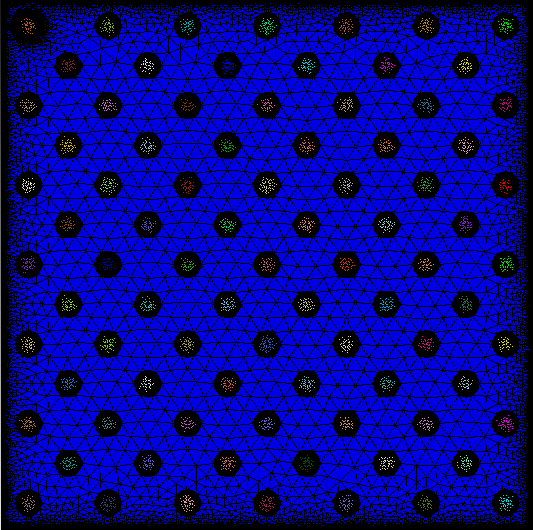
\includegraphics[scale=0.5]{fcc_mesh.png}
\caption{Meshed Xenon bubble inside U-10Mo matrix}
\label{fcc_mesh}
\end{figure}


\begin{figure}[H]
\centering
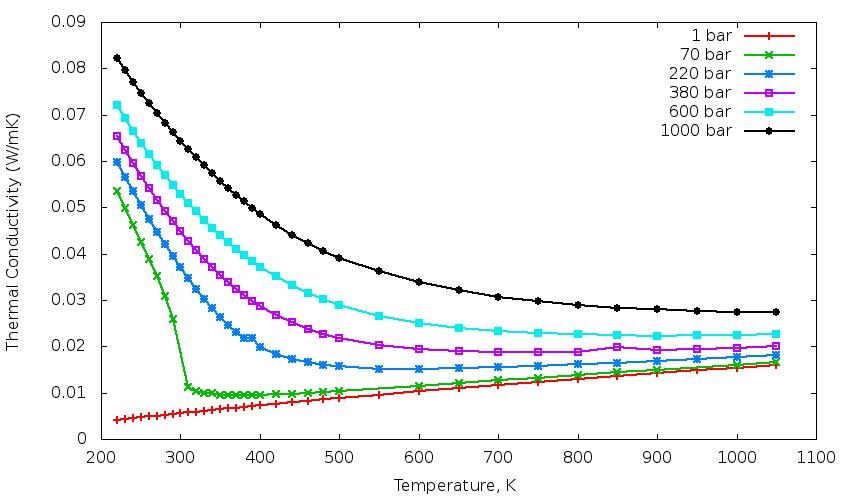
\includegraphics[scale=0.5]{Xe_K.png}
\caption{Thermal Conductivity of Xenon with increasing pressure}
\label{fig_Xe_K}
\end{figure}


\end{doublespacing}


\chapter{Results}
\section{Results}
\begin{doublespacing}


\end{doublespacing}


\chapter{Discussions and conclusions}

\begin{doublespacing}
The goals of this thesis were to explore the potential of RUS methods for long cylindrical tubes, study the contact pressure between the two cylinders in target, and the usefulness of this technique in assessing target damage due to radiation. The results obtained from RUS are highly dependent on the choice of the geometry. A finite element model was made to predict the frequency, based on geometry, density and elasticity matrix. After predicting the appropriate elastic constants, the RUS spectrum amplitude on different targets with different draw plug was studied. Experimental results from the contact pressure analysis was discussed. Theoretical study was completed to see the effect of radiation on mechanical properties of the material. After carefully studying the radiation effect on material, some recommendations can be made to use this technique properly  inside a hot cell. 

\section{Conclusion}
Experimentally detected frequency based on the quality factor is shown in Figure \ref{freq_Q}. Minimum frequency was detected  around 250 kHz. Theoretically, below 250 kHz some modes existed, but due to the length and weight of the sample all these mode frequencies had undetectable responses. In RUS, a Demarest plot is usually used to measure the experimental Poisson's ratio. However, to generate a complete Demarest plot, it is necessary to experimentally  detect first 20 modes. A time-of-flight method can be handy in this situation to measure Poisson's ratio for an isotropic material. Even though the finite element method  used in this study was highly time consuming, a simple mesh study was done to see the effect of the meshing on the eigen frequencies. A two pinducer system with a different holding mechanism was used to detect the frequencies below 250 kHz. But because of the size and shape of the sample the experiment was done in "surface to surface" manner. To extract all the frequencies below 300 kHz a study should be done to make a sophisticated detection system. To see the effect on the spectrum three different targets were made with three different plug sizes, which produced distinguishable responses.% Theoretical study was not done for this experiment. 

\section{Recommendations}
Based on the result discussed above, a couple of recommendations can be made. The importance of sophisticated measurement system has already been established. Machining of the sample is very important, any non-uniformity will produce discrepancies in the frequency response. Before using RUS to measure radiation effects, some parameters should be considered. Dimensional change can happen after irradiation (Figure \ref{dim_joyo}). Before making any RUS measurement it is necessary to measure the dimension properly. Temperature has profound effect on the elastic constants. So cooling down of the irradiated material, and proper heat treatment might be necessary for the sample. An experiment can be designed to  measure the contact resistance of the assembled targets. A numerical model of the assembled targets might help to understand the behavior of the RUS responses. 

\section{Future Work}
Future work in extending RUS method should involve looking at the development of a quantitative measurement system for contact pressure between two cylinders. Creating a correlation between the thermal contact resistance and amplitude of the target would help to mathematically explain the phenomena. This idea is based on the experimental results from target. To use RUS in radiation environment, inserting the whole setup in the hot cell is an important step. The transducer response in the radition field should be studied. Study of non-uniformity and anisotropy in the field of RUS may help in studying radiation damage with RUS.


\end{doublespacing}


\chapter{Acknowledgments}
\begin{doublespacing}
\section{Thermal Contact Resistance}
When two bodies come in contact, heat flows from the hotter to the colder body. A temperature difference is observed at the interface between the two surfaces in contact. The magnitude of the temperature drop is related to the \textit{thermal contact resistance} between the contacting surfaces. Thermal contact resistance is an effect due to surface roughness causing a temperature drop across the interface. These surface irregularities creates intermittent points of contact and air gap in the interface. The heat transfer is actually governed by both the conduction through the contact spots and conduction or convection/radiation across the gaps.
\begin{figure}[H]
\centering
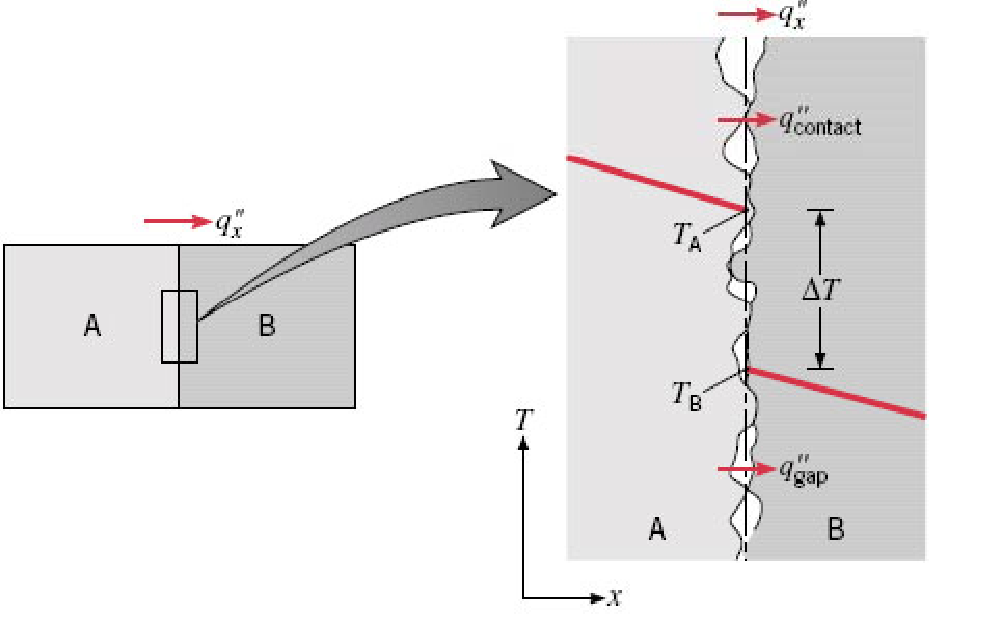
\includegraphics[scale=0.45]{contact_resistance}
\caption{Temperature drop due to thermal contact resistance}
\label{fig_contact_res}
\end{figure}

 \begin{equation}
 q_x^{''} = q_{contact}^{''} + q_{gap}^{''}
 \end{equation}
 \nomenclature{$q^{''}$}{heat transfer}
 
 Where $q_x^{''}$ is total heat transfer across the contacting surfaces. Figure \ref{fig_contact_res} shows temperature drop across the contact surface\cite{bergman2011fundamentals}. Thermal contact resistance is a function of the temperature difference due to surface imperfection and the heat transfer rate. This relationship can be shown in the following way.
 
\begin{equation}
\label{eq_contact_res}
R=\frac{\Delta T}{q_{x}^{''}}
\end{equation}
\nomenclature{$R$}{thermal contact resistance}

Where R is the thermal contact resistance and $\Delta T$ is the temperature difference across the interface of the two surfaces.

\section{Contact Pressure}
As discussed in the previous section heat transfer through the interfaces formed by the mechanical contact of two solids occurs in three forms: conduction through contacting spots, conduction through the gas-filled voids and radiation. In normal situations, radiation effects are small compared to the other two parameters. Another geometric parameter that controls the heat transfer through the contacting spots is the ratio of actual to apparent areas of contact. This ratio is called \textit{contact pressure} which is determined by \textit{relative contact pressure}. The relative contact pressure is defined as the ratio of applied pressure to the contact microhardness$(P/H_c)$. This relative contact pressure also plays an important role in the thickness of the air gap between the contacting interfaces. The ratio $P/H_c$ controls three geometric factors that control the heat transfer: contact spot density, mean contact spot radius, and separation distance of the mean planes of the two contacting surfaces \cite{song1988relative}. Contact microhardenss, $H_c$, depends on several parameters: mean surface roughness, method of surface preparation and applied pressure. An explicit relation was found in reference \cite{song1988relative} for the relative contact pressure 
\nomenclature{$P$}{applied pressure}
\nomenclature{$H_c$}{contact microhardness, MPa}
\nomenclature{$\sigma$}{RMS surface roughness}
\nomenclature{$c_2$}{Vickers correlation coefficient}
\nomenclature{$k$}{harmonic mean conductivities}
\nomenclature{$h_c$}{contact conductance, $W/m^2K$ }
\nomenclature{$tan\theta$}{mean absolute slope of the surface profile}

\begin{equation}
\label{eq_contact_pres}
\frac{P}{H_c} = \left[\frac{P}{(1.62\times10^6 \sigma/m)^{c_2}} \right ]^\frac{1}{1+.071c_2}
\end{equation}
Here $\sigma$ is the RMS surface roughness and $c_2$ is the Vickers correlation coefficients.


\begin{figure}[H]
\centering
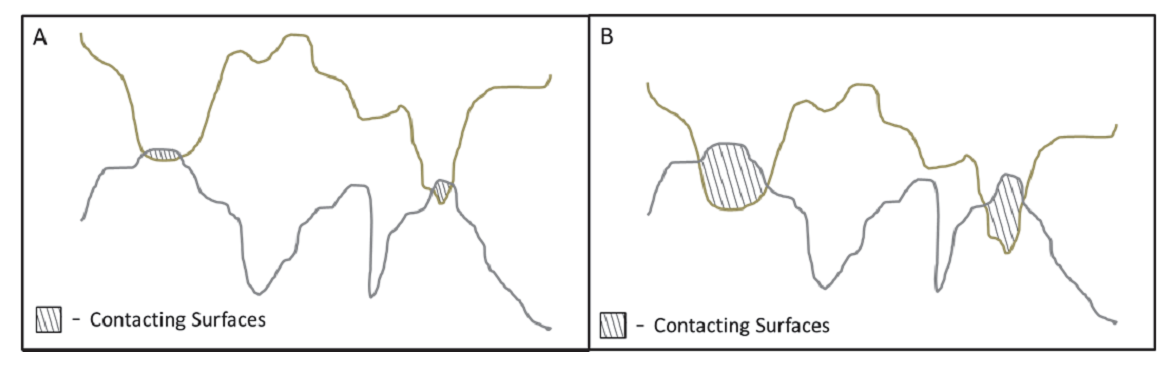
\includegraphics[scale=0.4]{contact_pressure}
\caption{Magnified profile of two surfaces in contact with changing contact pressure(A)less contact pressure (B)higher contact pressure}
\label{fig_contact_pressure}
\end{figure}

Figure \ref{fig_contact_pressure} shows the change of contacting surface based on the contact pressure. Consequently it will also change the thermal contact resistance. In the context of Molybdenum-99 targets contact pressure plays an important role in design \cite{philip}, and choosing appropriate forming pressure. Reducing the contact resistance is one of the major challenges of designing the target. Low contact resistance will help to remove heat throughout the irradiation process  which is necessary for the safety of the target. It is not possible to experimentally determine the actual contact pressure between the surfaces. For plastically deformed surfaces Yovanovich \cite{madhusudana1996thermal} proposed the following correlation for thermal contact conductance :

\begin{equation}
\label{eq_yavonovich}
\frac{h_c \sigma}{k tan\theta} = 1.25 \left( \frac{P}{H_c}\right)^{0.95}
\end{equation}
Here $h_c$ is solid spot conductance, $tan\theta$ is the mean absolute slope for the surface profile and k is the harmonic mean conductivities of the two contacting surfaces.


%Yovanovich et el \cite{yo6novich1982surface} developed an %implicit geometric model that relates relative contact pressure %with surface roughness. For plastically deforming asperities %whose 


\section{Experiment}
\subsection{Target Assembly}
This particular experiment was designed to investigate the effect of different contact pressures effect on the RUS spectrum. To characterize the contact pressure between two concentric cylinders, three different targets were made using three different draw plug sizes without any foil. Since three different plug sizes were used to make three different targets, the contact pressures are different in each target. The draw plug assembly procedure was used to make the targets (Figure \ref{draw_plug}). The draw plug target manufacturing method or drawing process uses a die and plug to mechanically expand the inner tube while holding the outer tube in steady. The two aluminum tubes cut to a specified length are pre-manufactured (with proper tolerance) so that inner tube can slide freely into the outer tube. 

Once the tubes have been slid together, they are placed in a die that confines the outer tube in the drawing process. A hydraulically driven rod with a plug attached to the end is then forced through the inner tube. The size of the plug is important because it deforms the inner tube plastically, and thus reduces the gape between the two cylinders. Increasing the plug size will increase the deformation that occurs in the inner tube (aluminum) leading to an increase in contact pressure. Figure \ref{draw_plug} shows the draw pug set up for target manufacturing. 
%...........put a picture in this spot

\begin{figure}[H]
\centering
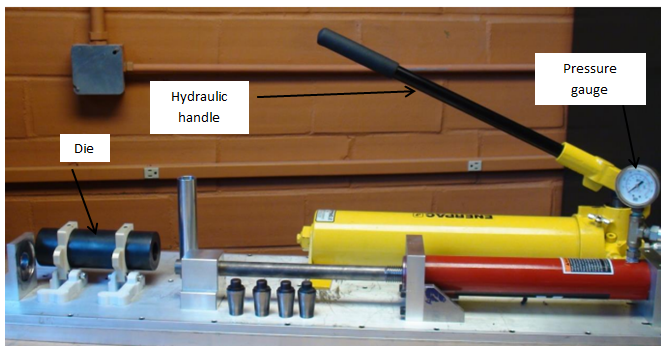
\includegraphics[scale=0.7]{drawplug_1} 
\caption{Draw plug Rig }  
\label{draw_plug} 
\end{figure}

As mentioned earlier, the inner tube deforms plastically as the plug is drawn though.  The outer tube deforms elastically. During the manual process of drawing the plug through the inner tube, the formation (drawing) pressure was recorded. This is the required pressure to drive the plug through the target which is not an actual forming pressure, but it provides a qualitative idea about the deformation. Higher forming pressure means higher deformation.

\begin{table}[H]
\caption{Weights of the three different targets}
\centering
\begin{tabular}{c|c|c|c}
\hline\hline
 Draw plug ID & Plug Outer Diameter (m) & Tube Length (m) & Target Mass (g)  \\
\hline
 48 & 0.02662 & 0.161 & 61.470 \\
 \hline
 49 & 0.02664 & 0.161 & 60.942 \\
 \hline
 50 & 0.02667 & 0.161 & 61.213 \\
 \hline
\end{tabular}
\label{plug_mass}
\end{table}

 \begin{figure}[H]
 \centering
 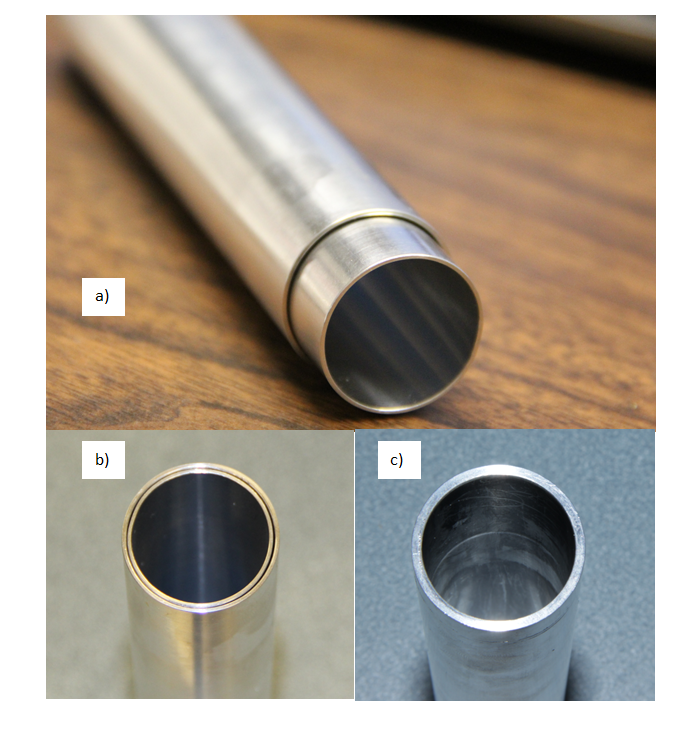
\includegraphics[scale=0.5]{tubes_target_bfore}
 \caption{a)Inner and Outer tubes together b)Two concentric cylinders before deformation c)After assembling the target}
 \label{fig_tubes_target}
 \end{figure}

 Forming pressure for the two plugs (48 and 50 ) is shown in Figure \ref{p_48_50}. As  can be seen from the plot that forming pressures are also different for different plugs along the distance of the target, but they have a similar  trend. At the beginning of the process the required pressure is higher. 

\begin{figure}[H]
\centering
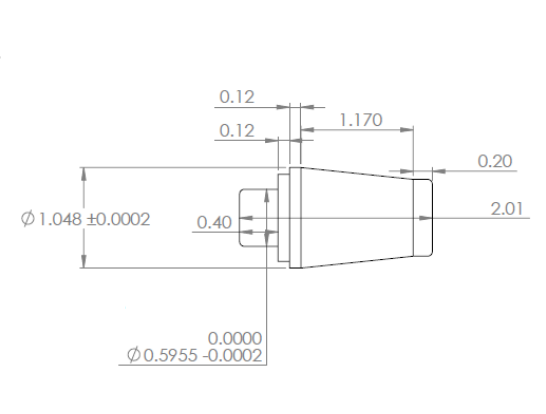
\includegraphics[scale=0.7]{plug_48_fig}
\caption{Dimensions(inches) of a draw plug(48)}
\label{fig_plug48}
\end{figure}


 
 
\begin{figure}[H]
	\subfloat[ plug 48 \label{p_48}]{%
	  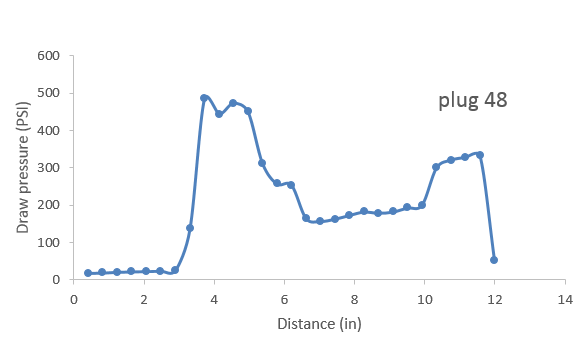
\includegraphics[scale=0.6]{p_48_psi}}
	\hfill
	\subfloat[plug 50 \label{p_50}]{%
	 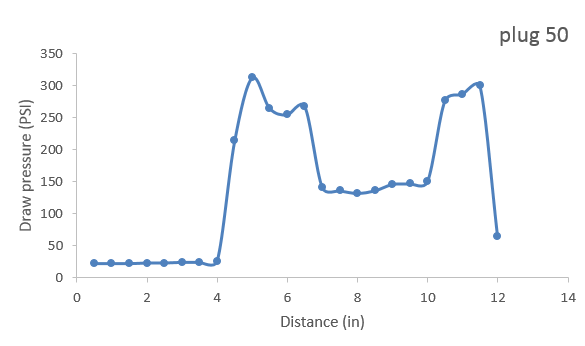
\includegraphics[scale=0.6]{p_50_psi}
	}
	\caption{Plot of pressure during swagging using two different plug sizes}
	\label{p_48_50}
\end{figure}

\newpage
\subsection{Results}

The purpose of this experiment was to detect variations in RUS spectrum in different contact pressures which is related to thermal contact resistance. Since three different draw plugs were used (plug 48, 49 and 50), it is assumed that the targets have three different contact pressures. The outer  diameter of the plugs are shown in Table \ref{plug_mass}. 

 To evaluate the RUS responses of the targets, the spectrum of the individual tube (inner and outer) is studied. The spectrum of the outer tube is shown in Figure \ref{outer_tube}. The inner tube also shows the same type of response (Figure \ref{fig_inner_tube}). All three tubes show a similar pattern. At around $8.3\times10^5$ Hz there is a response around $0.9\times10^{-4}$ volts. The amplitude of the peaks is considered for this experiment. Since the geometry is a hollow cylindrical and the mass is constant before and after making the target, the only variable will be the amplitude.


\begin{figure}[H]
\centering
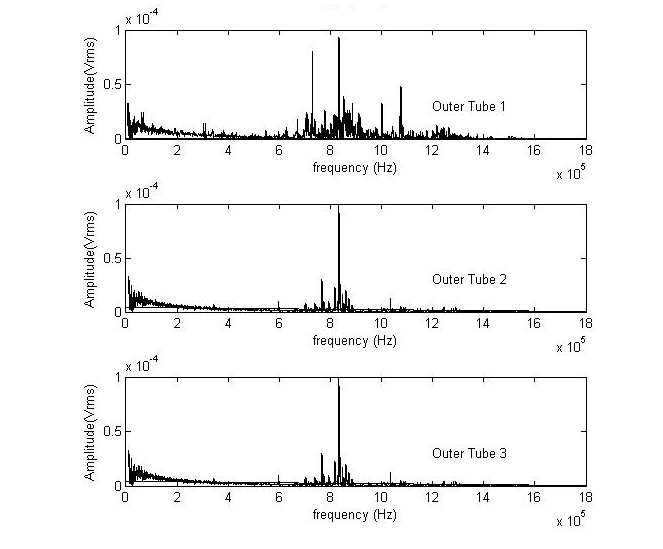
\includegraphics[scale=0.8]{outer_tube} 
\caption{RUS spectrum of the outer tube}  
\label{outer_tube} 
\end{figure}
The diameter of the plug varies from $0.02662$ m to $0.02667$ m . These different plug sizes will exert different pressures in the inner tubes. As the plug size increases, it will cause more plastic deformation on the inner tube. 
Given the sizes of the plugs it is assumed that only the inner tube is plastically deformed \cite{annemarie}. Outer tube's deformation is elastic.  Mass of the object plays an important role in response of the of the amplitude. The masses of the three different targets are in Table \ref{plug_mass} . \\[0.5 in]



\begin{figure}[H]
\centering
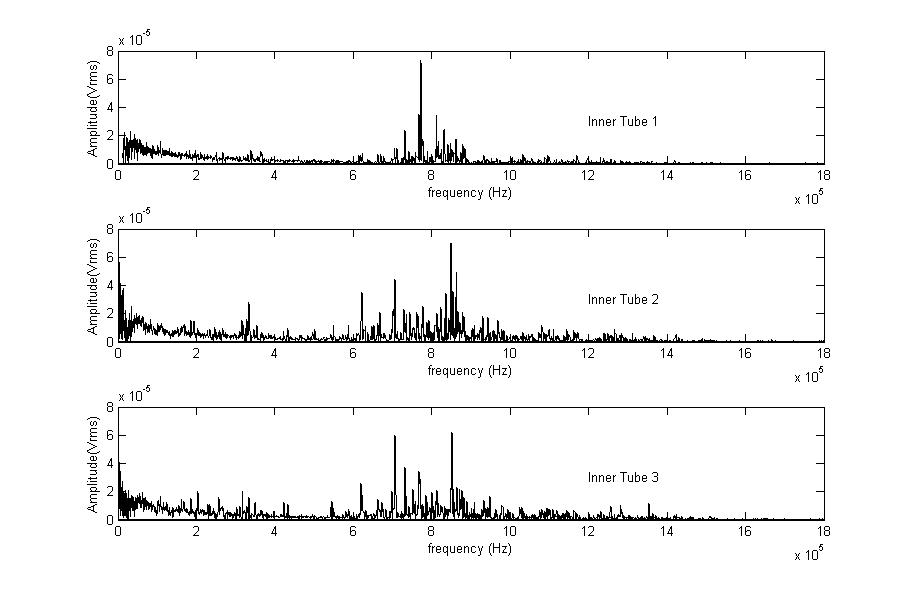
\includegraphics[scale=0.5]{all_inner_tube}
\caption{RUS spectrum of the inner tube}
\label{fig_inner_tube}
\end{figure}

The experimental findings of the RUS of the three different assembled targets are shown in Figure \ref{target_rus}. \\[0.3 in]
\begin{figure}[H]
\centering
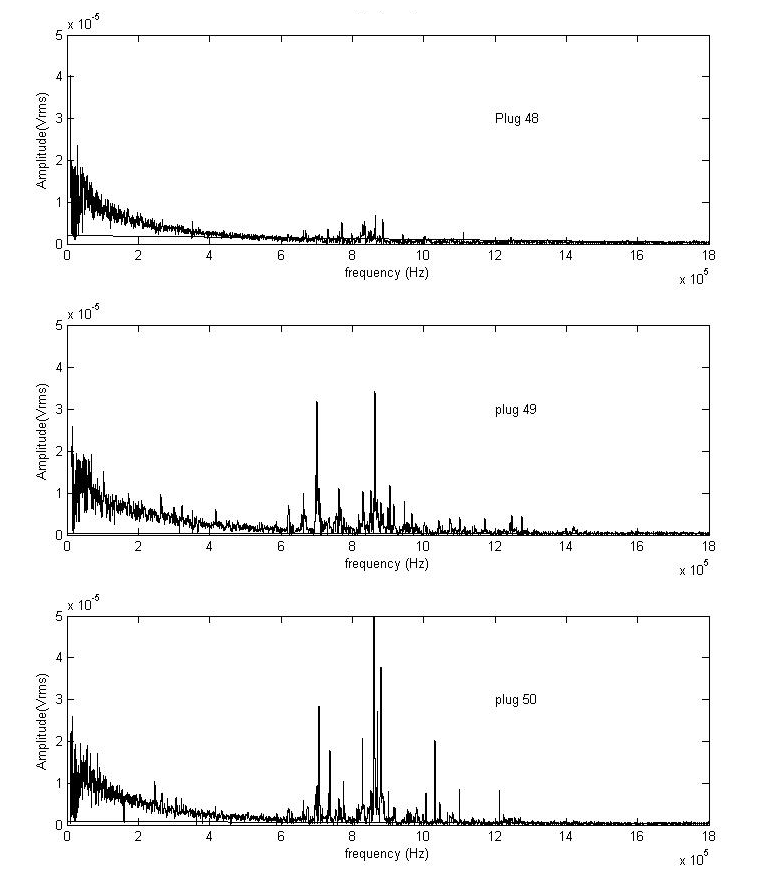
\includegraphics[scale=0.5]{3plut_plot_different_plug} 
\caption{RUS spectrum of the targets}  
\label{target_rus} 
\end{figure}

Figure \ref{target_rus} shows the RUS response for three different targets. The frequency range that we are interested in is $6.5$ to $10\times Hz$. In this frequency range the amplitudes vary significantly. The result can be summarized in Table \ref{amplitude_plug}.  \\[0.3 in]
\begin{table}[H]
\caption{Highest amplitudes in the interested frequency zone }
\centering
\begin{tabular}{c|c|c}
\hline\hline
Draw plug size & frequency range $(\times 10^5) Hz$ & Amplitude $(V_{rms}\times 10^{-5}) volts$\\
\hline
48 & 6.5-9 & 1 \\
49 & 6-10 & 3.5 \\
50 & 6-10 & 5 \\
\hline
\end{tabular}
\label{amplitude_plug}
\end{table}



The differences in the amplitudes of spectrum can be explained using the contact pressure between the two cylinders. Since the inner tube plastically deformed with three different radii, contact pressures are different in these targets. The RUS setup used to excite and measure the frequency spectrum is same as Figure \ref{rus_setup}. As the draw plug size increases the response amplitudes increases. From Figure \ref{rus_setup}, only the outer tube is excited and the receiving transducers are receiving signals from the outer tube. Since the masses of these targets are almost the same (Table \ref{plug_mass}), the amplitude depends on the modes that are being produced. Since aluminum is used for both inner and outer tube, surface roughness does not change for the deformed targets. The only variable that can influence the response in RUS has to be \textit{contact pressure} (Equation \ref{eq_yavonovich}). 

%If the contact pressure is low, the inner tube will damp the %vibration of the outer tube. If they are pressed tightly, their %resonance amplitude will not diminish as much, as can be seen %from the experiment. The reproducibility of the spectrum of the %targets was also studied.

\begin{figure}[H]
%\centering
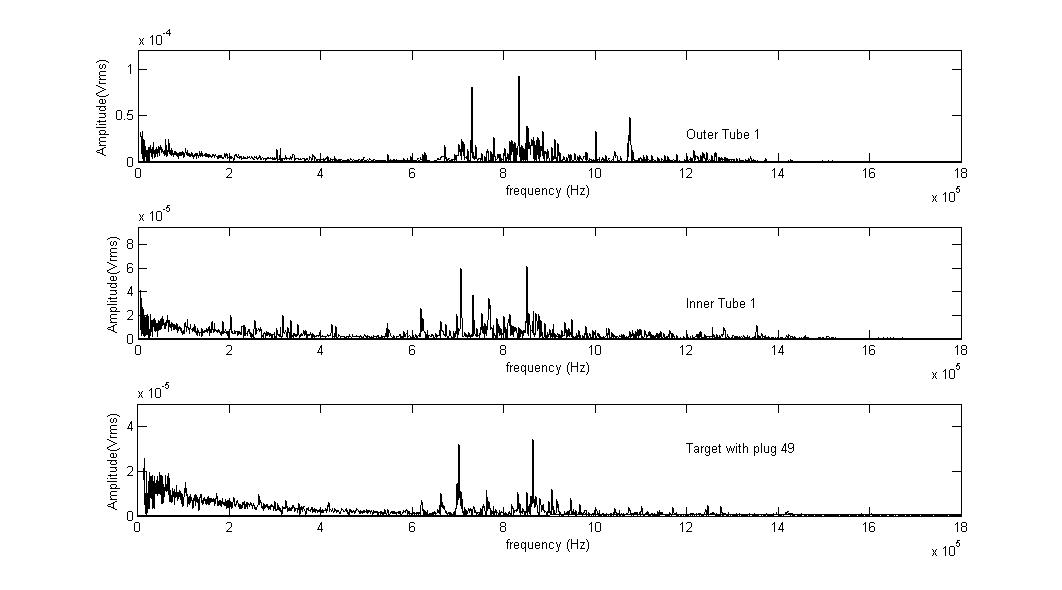
\includegraphics[scale=0.4]{3tubes_plot}
\caption{RUS spectra of outer tube, inner tube and one of the targets}
\label{fig_3_diff_tubes}
\end{figure}

Figure \ref{fig_3_diff_tubes} shows that outer tube has a response around $1\times 10^{-4} V$ and the inner is around $0.8 \times 10^{-4} V$. When they are pressed together with draw plug 49, the response reduced to around $0.4\times 10^{-4} V$ . All the individual tubes' (inner and outer) response were examined before they were deformed to a target. 



\end{doublespacing}






\printbibliography


\appendix

\chapter{XYZ Algorithm}
\begin{lstlisting}

clc
clear all
NN=input('Input the value of N');
%-----next 13 lines assign an index IG to each basis function
C=zeros(3,3,3,3);
IG=0;
for I=1:3
   for L=1:NN+1
      for M=1:NN+1
         for N=1:NN+1 
          if (L+M+N > NN+3), break, end
          IG=IG+1;
          IC(IG)=1;
          LB(IG)=1;
          MB(IG)=1;
          NB(IG)=1;
             
         end
      end
   end
    
end
rank=0.5*(NN+1)*(NN+2)*(NN+3);
NR=IG;
Gamma=zeros(rank,rank);
for IG=1:NR
    for JG=IG:NR
       I=IC(IG);
       J=IC(JG);
       LS=LB(IG)+LB(JG);
       MS=MB(IG)+MB(JG);
       NS=NB(IG)+NB(JG);
       
       Gamma(IG,JG)=C(I,1,J,1)*LB(IG)*LB(JG)*func(LS-2,MS,NS)+...
           C(I,2,J,2)*MB(IG)*MB(JG)*func(LS,MS-2,NS)+...
           C(I,3,J,3)*NB(IG)*NB(JG)*func(LS,MS,NS-2)+...
           C(I,1,J,2)*LB(IG)*MB(JG)+...
           C(I,2,J,1)*MB(IG)*LB(JG)*func(LS-1,MS-1,NS)+... 
           C(I,1,J,3)*LB(IG)*NB(JG)+...
           C(I,3,J,1)*NB(IG)*LB(IG)*func(LS-1,MS,NS-1)+...
           C(I,2,J,3)*MB(JG)*NB(IG)+...
           C(I,3,J,2)*NB(IG)*MB(JG)*func(LS,MS-1,NS-1);
       Gamma(JG,IG)=Gamma(IG,JG);
     if(I==J) E(IG,IG)=func(LS,MS,NS) ; 
       end  
    end   
    end

    
    [vects vals]=eig(E\Gamma);
    
    
    
    



\end{lstlisting}


\end{document}





